\chapter*{Appendix}
\addcontentsline{toc}{chapter}{Appendix}
\section*{List of appendices}
\vspace{-8em}

% vor \listofanhang müssen Einrückungen angepasst werden
\abstaendeanhangverzeichnis

\listofanhang
\clearpage
\spezialkopfzeile{Attachement} % damit in der Kopfzeile das Wort "Anhang" angezeigt wird

\anhang{So funktioniert's}

\lstset{language=TeX, % hervorzuhebende Keywords definieren
  morekeywords={anhang, anhangteil}
}


Um den Anforderungen der Zitierrichtlinien nachzukommen, wird das Paket \verb|tocloft| verwendet. Jeder Anhang wird mit dem (neu definierten) Befehl \lstinline|\anhang{Bezeichnung}| begonnen, der insbesondere dafür sorgt, dass ein Eintrag im Anhangsverzeichnis erzeugt wird. Manchmal ist es wünschenswert, auch einen Anhang noch weiter zu unterteilen. Hierfür wurde der Befehl \lstinline|\anhangteil{Bezeichnung}| definiert.

\anhangteil{House of Prototyping Guidelines: Prototyping Dimensions}\label{attachement:prototyping_dimensions}
\begin{figure}[htb]
\centering
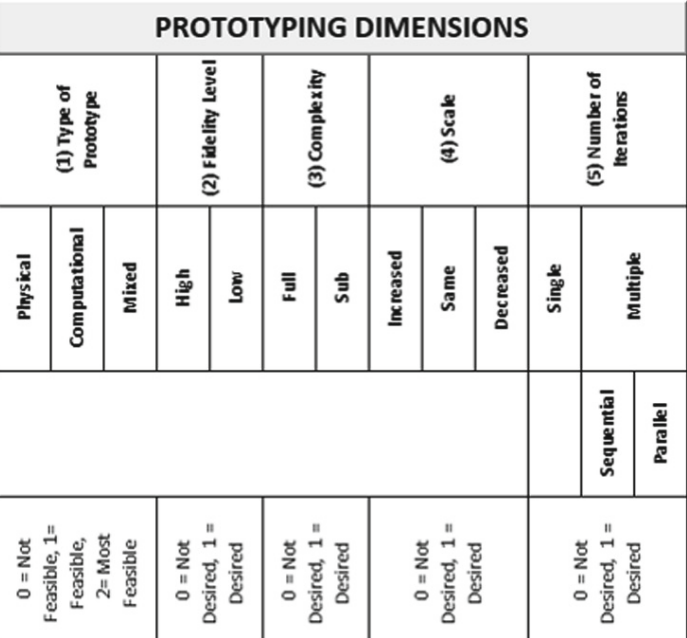
\includegraphics[width=0.9\linewidth]{graphics/Prototyping_dimensions.png}
\caption{Prototyping Dimensions to categorize prototypes}
\end{figure}


